\chapter{System Design and Implementation}\label{ch:implementation}
The system pipeline\footnote{See footnote on page~\pageref{foot:pipe}} consists of three separate processes:
preprocessing of the Czech News dataset~\ref{sec:data-preprocessing}, feature extraction~\ref{sec:feature-extraction},
and evaluation~\ref{sec:evaluation}.

The algorithm is implemented in \textit{Python} programming language.
Libraries \textit{NumPy} and \textit{PyTorch}~\cite{PyTorch} are extensively used throughout the whole project.

\section{Preprocessing of the Czech News Dataset}\label{sec:data-preprocessing}
\begin{wrapfigure}[7]{r}{0pt}
    \centering
    \raisebox{0pt}[\dimexpr\height-0.831\baselineskip\relax]{%
    \begin{forest}
        for tree={
        font=\ttfamily,
        grow'=0,
        child anchor=west,
        parent anchor=south,
        anchor=west,
        calign=first,
        edge path={
        \noexpand\path [draw, \forestoption{edge}]
        (!u.south west) +(7.5pt,0) |- node[fill,inner sep=1.25pt] {} (.child anchor)\forestoption{edge label};
        },
        before typesetting nodes={
        if n=1
        {insert before={[,phantom]}}
        {}
        },
        fit=band,
        before computing xy={l=15pt},
        }
        [dataset
        [name1
        [image1\_128x128.jpg]
        [image2\_128x128.jpg]
        [image3\_128x128.jpg]
        ]
        [name2
        [image1\_128x128.jpg]
        [image2\_128x128.jpg]
        ]
        [\ldots]
        ]
    \end{forest}
    }
    \caption{Standard image dataset format}
    \label{fig:dataset}
\end{wrapfigure}
The goal of preprocessing is to convert the input dataset (Czech News~\ref{subsec:czenew}) to the standard format.
The standardized dataset consists of directories with each directory representing one identity/label.
In these directories, there are images corresponding to the identity.
In this case, the images contain faces in different positions.

The desired format is visualized in figure~\ref{fig:dataset}.
\newpage
As I mentioned in the dataset description~\ref{subsec:czenew}, the area containing face was selected by human.
Because of that, the geometry of the area is not always consistent.
This significantly decreases the model performance.
For this reason, as is described in the section~\ref{subsec:preproalgo}, this reference position is not
used directly in the algorithm.

\subsection{Preprocessing Algorithm}\label{subsec:preproalgo}
Before the presentation of the algorithm it is necessary to define "Intersection over Union (IoU)."
As the name implies, IoU is computed as a fraction with intersection area in the numerator and union area in the
denominator (see figure~\ref{fig:iou}).
\begin{figure}[H]
    \centering
    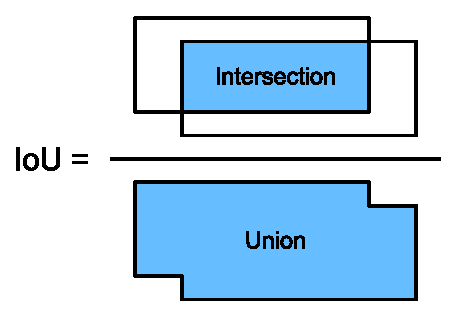
\includegraphics{images/implementation/iou.eps}
    \caption{IoU visualization\cite{IoU}}
    \label{fig:iou}
\end{figure}
In the context of face detection each area is defined by a corresponding bounding box.

The preprocessing algorithm consists of seven steps:
\begin{enumerate}
    \item First, I iterate over the annotation files.
    \item Then I iterate over the names and detections within the file.
    \item In the third step, I fetch the frame out of the video corresponding to the detection.
    \item \label{itm:pre4} Then I detect all the faces in the frame using MTCNN detector.
    The detector returns coordinates of the bounding boxes\footnote{See footnote on page~\pageref{foot:bbox}} and the
    facial landmarks\footnote{Salient regions of the face.}.
    \item \label{itm:pre5} I select the detection which meets the following two conditions:
    \begin{enumerate}
        \item has the biggest IoU with reference of all the detections;
        \item the IoU value is at least \textbf{0.5} (This value has been determined experimentally as
        is described in the section~\ref{subsec:detection-mislabelings}.).
    \end{enumerate}
    If these conditions are not met for any of the detections the frame is omitted.
    \item At this point I perform face frontalization using the facial landmarks from step~\ref{itm:pre4} to the
    predetermined reference position.
    This is achieved by using the least squares method to find an affine transformation\footnote{A function between
    affine spaces which preserves points, straight lines and planes.} between the two sets of coordinates.
    Applying the transformation results in an image with facial landmarks in the similar position as the reference.
    To carry out the transformation \textit{OpenCV} library is used.
    The implementation in this library allows for specification of the output size.
    I specified the output as $128 \times 128$ pixels because it is the input size of the ResNet-18 model.
    \item In the last step, I save the image to a location defined by the standardized dataset format
    (\path{dataset/name/image_128x128.jpg}).
\end{enumerate}

The processed dataset contains 791 identities and 478529 images.
The conditions in step~\ref{itm:pre5} were not met 254078 times.
This resulted in the loss of the same amount of images and 447 identities.
While the loss seems to be significant, the resulting amount of images is sufficient for system evaluation.

Having the dataset in the desired format we can proceed with feature extraction.

\section{Feature Extraction}\label{sec:feature-extraction}
Feature extraction~\cite{FeEx} is a process of dimensionality reduction by which an initial set of raw data
is reduced to the set of feature vectors.
In this study this process is carried out by feeding the input image $x_i \in \mathbb{R}^{128\times128 }$ to the CNN model.
On the output we retrieve a feature vector $y_i \in \mathbb{R}^{1024}$.

The model used is 18-layer ResNet~\ref{subsec:resnet} which was trained under a supervision of the ArcFace loss.
The training process was not executed as part of this study since the trained model is freely available online.
The model was downloaded from the ArcFace implementation repository~\cite{ArcFacePyTorch}.
The information about the dataset on which the model was trained is unknown.

\subsection{Feature Extraction Algorithm}\label{subsec:feexalgo}
The feature extraction algorithm consists of 6 steps:
\begin{enumerate}
    \item iterate over the images in the dataset;
    \item save the image and the flipped version into an array with shape $2\times1\times128\times128$;
    \item feed the array to the ResNet-18 model;
    \item retrieve the feature vector on the output;
    \item save the vector along with the corresponding label into an array;
    \item once all the feature vectors are computed, save the resulting array using the \textit{h5py} module.
\end{enumerate}

In the final array there are 478529 feature vectors (the number of images in the processed dataset).
The whole file is approximately 2 GB in size.

Having the feature vectors computed, we can carry out the evaluation~\ref{sec:evaluation}.

\section{Evaluation}\label{sec:evaluation}
The system's performance is evaluated on the verification task.
The task consists of computing cosine distance between every two feature
vectors and deciding, given some threshold, whether the vectors correspond to the same identity ot not.
This computation is carried out for all the threshold values in the specified interval.

The algorithm is described in depth in the following section~\ref{subsec:thresholding-algorithm}.

\subsection{Thresholding Algorithm}\label{subsec:thresholding-algorithm}
First, I would like to analyze the algorithm time complexity and memory demands.

As I previously mentioned, it is necessary to compute the distances between every two feature vectors in the dataset.
The number of vector pairs is equal to
\begin{equation}
    N_{pairs} = \frac{n\left(n+1\right)}{2} = \frac{478529\left(478529+1\right)}{2} \approx 114.50 \cdot 10^9,
\end{equation}
where $n = 478529$ is the number of vectors in the dataset.
If we computed all the distances using optimized matrix operations at once, we would need at least 460 GB of RAM memory.

Given that the algorithm time complexity is $O(n^2)$ and the big memory demands, it was desirable to split the distance
matrix into smaller sub-matrices.
Splitting the matrices allows for parallel processing as the sub-matrices can be processed on different CPU cores.
This significantly reduced the computation time.
My approach made the use of optimized matrix libraries possible while reducing the excessive memory demands.

There are 5 steps in the parallelized algorithm:
\begin{enumerate}
    \item Initially, I generate all the interval pairs.
    \item In the second step, I pass the intervals as an argument to the generator function.
    This function returns pairs of slices of the feature vector array and corresponding labels.
    \item Next, I pass the generator function as an argument to the \textit{imap} method from \textit{multiprocessing}
    module.
    This method iterates over the generator function and passes the retrieved values to separate processes.
    With this step, parallelized processing is achieved.
    \item In the fourth step, the matrix of cosine distances is computed between the two feature vector arrays
    and two label arrays using \textit{cosine\_distances} method from \textit{sklearn} library~\cite{scikit-learn}.
    Computing the matrix for labels allows for simple and efficient comparison of predictions and reference
    values using matrix operations.
    \item Next, I convert the matrices to two long vectors.
    \item Now I iterate over the list of threshold values ($\left[ 0, 0.05, 0.10, 0.15, \ldots 2 \right]$).
    \item I apply the threshold to the distances.
    This way I retrieve a vector of binary values.
    \item I use the methods \textit{sum} and \textit{logical\_and} along with elementwise binary value inversion to
    count the number of \textit{true positives (TP)}, \textit{true negatives (TN)}, \textit{false positives (FP)} and
    \textit{false negatives (FN)}.
    \item In the last step, I do elementwise summation of the arrays which were returned from the parallel processes.
\end{enumerate}

The output of the algorithm is an array with 200 rows and 4 columns.
The rows correspond to the threshold values; columns to \textit{TP}, \textit{TN}, \textit{FP} and \textit{FN}.

Having all these values accumulated we can proceed with computation of all the relevant metrics.

\subsection{System Evaluation}\label{subsec:syseval}
In order to evaluate the performance, I implemented an algorithm which computes precision~\ref{sec:precision},
recall~\ref{sec:recall} and $F_1$ score~\ref{sec:f-score} on the data from the previous section.
The system is evaluated on LFW~\ref{subsec:lfw} and processed Czech News dataset~\ref{subsec:czenew}.
In figure~\ref{fig:prft} there is a progression of these metrics.

We can see that in comparison with LFW dataset the system achieved 6 \% higher performance on the processed
Czech News dataset.

LFW dataset was not aligned using the preprocessing algorithm described in section~\ref{sec:data-preprocessing},
which leads to a slightly different positions of faces than what the model is used to.
This is probably the reason for the low $F_1$ score on the dataset.

\begin{figure}[H]
    \begin{subfigure}{\textwidth}
        \centering
        \includegraphics[width=0.95\columnwidth]{images/implementation/prft_lfw-align-128.eps}
        \caption{LFW dataset~\ref{subsec:lfw}}
        \label{fig:prft_arcface_lfw}
    \end{subfigure}

    \begin{subfigure}{\textwidth}
        \centering
        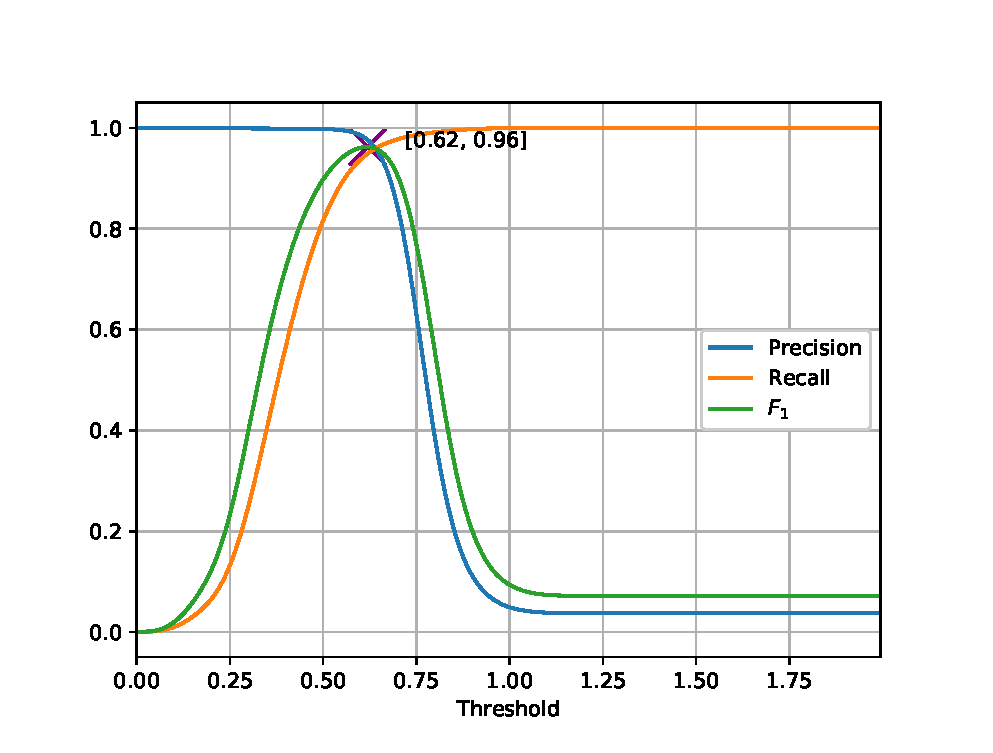
\includegraphics[width=0.95\columnwidth]{images/implementation/prft_fav-128_N1.eps}
        \caption{Processed Czech News dataset~\ref{subsec:czenew}}
        \label{fig:prft_arcface_cze}
    \end{subfigure}
    \caption{Progression of precision, recall and $F_1$ score with increasing threshold values. The metrics were
    computed on the outputs of my system based on ResNet-18.}
    \label{fig:prft}
\end{figure}


\subsubsection{Comparison with Commercial System}\label{subsubsec:performance-comparison}
In figure~\ref{fig:prft_eyedea} there is a similar chart as the one above.
The difference is, that the values were computed on the outputs of EyeFace SDK~\ref{subsec:eyeface}.

By comparing the chart below with chart~\ref{fig:prft_arcface_cze} we can see that the custom implementation
surpassed the commercial system by two percents.

\begin{figure}[H]
    \centering
    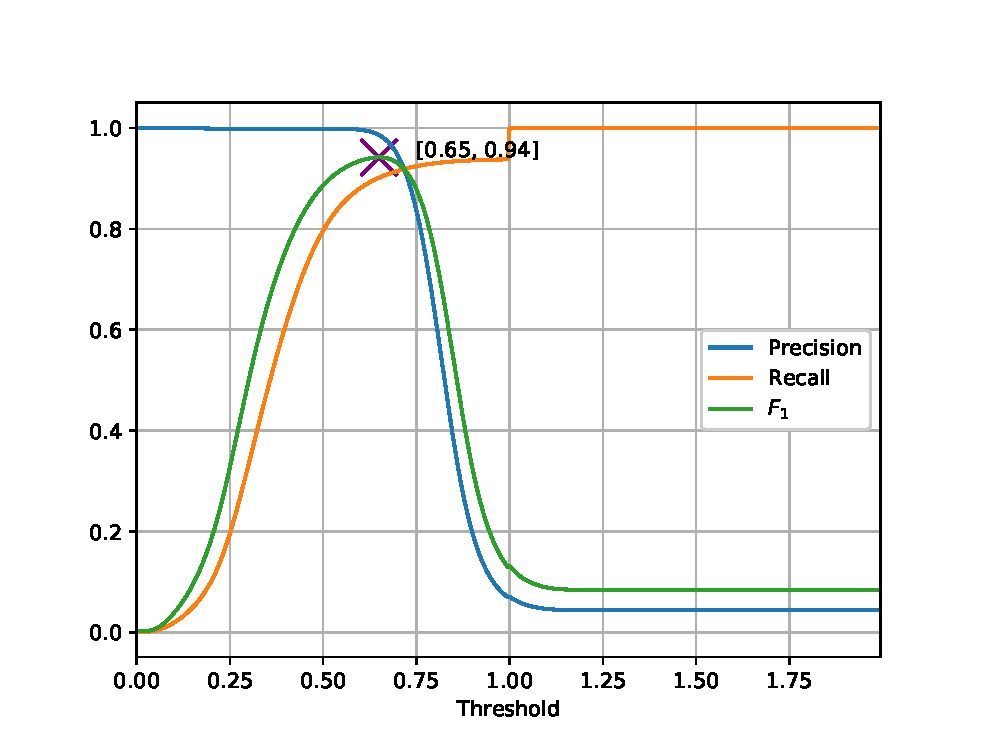
\includegraphics[width=0.95\columnwidth]{images/implementation/prft_eyedea.eps}
    \caption{Progression of precision, recall and $F_1$ score with increasing threshold values. The metrics were
    computed on the outputs of commercial system (EyeFace SDK~\ref{subsec:eyeface}) from the Czech News
    dataset~\ref{subsec:czenew}.}
    \label{fig:prft_eyedea}
\end{figure}

\subsection{Detection of Mislabelings}\label{subsec:detection-mislabelings}
As I mentioned in the section~\ref{sec:precision}, the precision curve can be used to detect incorrect labels in the
dataset.
In figure~\ref{fig:faulty_prft} there are three functions dependent on the threshold.

\begin{figure}[H]
    \centering
    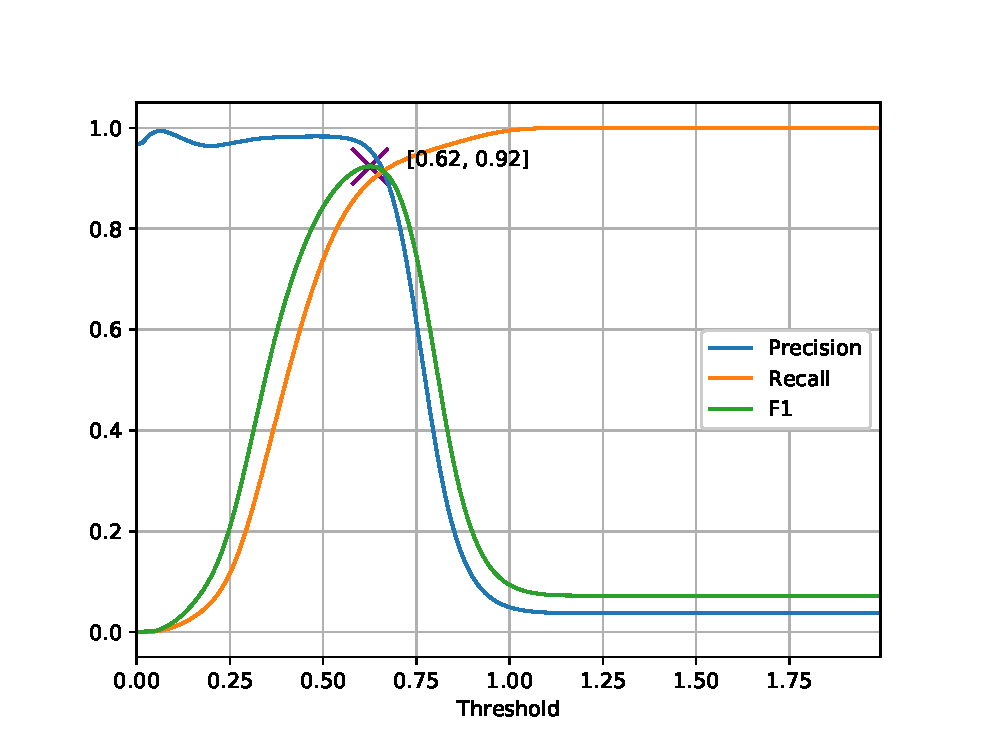
\includegraphics[width=0.95\columnwidth]{images/implementation/faulty_prft.eps}
    \caption{An example of precision curve~\ref{sec:precision} computed on a dataset containing errors.}
    \label{fig:faulty_prft}
\end{figure}

By the definition of precision ($Precision = \frac{TP}{TP+FP}$), there should not be any false positives
for threshold 0 because in such a setting, the system is strongly biased towards false negatives.
With this in mind, precision value which is not equal to 1 for threshold 0 is a sign of error.
This error can either reside in the dataset, or in the model.
If the error is in the dataset, it means that there are mislabelings.
If it is in the model, the whole system is faulty.

\begin{figure}[H]
    \centering
    \includegraphics[width=0.9\columnwidth]{images/implementation/faulty_detection.jpg}
    \caption{An example of a faulty detection.}
    \label{fig:faulty_bbox}
\end{figure}

This property of precision was used extensively during the experimentation.
Figure~\ref{fig:faulty_bbox} is an example of faulty face detection.
Because of the white stripe, the man in the foreground was not detected by the MTCNN detector selecting the bald man
on the right instead.
This led to an error in the dataset.
This issue was fixed by putting IoU threshold in place during the data preprocessing~\ref{sec:data-preprocessing}.

\subsection{Face Detector Evaluation}\label{subsec:detectorevaluation}
In order to evaluate the detector, I've implemented an algorithm which computes recall~\ref{sec:recall} on the IoU
values between the MTCNN detection and the area selected by human.
The process is very similar to the one described in section~\ref{subsec:thresholding-algorithm}.

The output is visualized in the image~\ref{fig:iou}.

The fact that recall ($\frac{TP}{TP+FN}$) never gets close to 1 is indicative of significant amount of
\textit{false negatives}.
To say it in other words, there are plenty of cases in which the face is not detected at all.

The value marked by purple cross is the threshold value set in the data processing pipeline~\ref{subsec:preproalgo}.
The big drop in recall for thresholds in range $\left< 0.4, 0.5 \right>$ is caused by not accepting the detections
of neighboring faces~\ref{fig:faulty_bbox} as \textit{true positive}.
With this in mind, higher recall value doesn't necessarily mean better performance.

\begin{figure}[H]
    \centering
    \includegraphics[width=0.95\columnwidth]{images/implementation/mtcnn_recall_fav-128_N1.eps}
    \caption{Recall computed on IoU~\ref{fig:iou} values.}
    \label{fig:mtcnn_recall}
\end{figure}

The selection of neighboring face as \textit{true positive} is exacerbated by the penchant of humans to select larger
area as containing the face.
To verify this hypothesis, I implemented a script which computes the average ratio of the area selected by human
to that of the detector.
The resulting ratio is \textbf{1.59}.
This means that human selects on average an area which is \textbf{59 \% larger} than the one selected by the detector.